\documentclass[a4paper]{article}
%Tutti gli usepackage vanno qui

\usepackage{geometry}
\usepackage[italian]{babel}
\usepackage[utf8]{inputenc}
\usepackage[T1]{fontenc}
\usepackage{tabularx}
\usepackage{longtable}
\usepackage{hyperref}
\usepackage{enumitem}
\hypersetup{
	colorlinks=true,
	linkcolor=black,
	filecolor=magenta,      
	urlcolor=blue,
}
% Numerazione figure 
\let\counterwithout\relax
\let\counterwithin\relax
\usepackage{chngcntr}

\counterwithin{table}{subsection}
\counterwithin{figure}{subsection}

\usepackage[bottom]{footmisc}
\usepackage{fancyhdr}
\usepackage{titlesec}
\setcounter{secnumdepth}{4}
\usepackage{amsmath, amssymb}
\usepackage{array}
\usepackage{graphicx}

%\usepackage{float}
\usepackage{layouts}
\usepackage{float}
\usepackage{eurosym}


\usepackage{layouts}
\usepackage{float}
\usepackage{eurosym}

%Comandi di impaginazione uguale per tutti i documenti
\pagestyle{fancy}
\lhead{
\includegraphics[scale=0.07]{res/images/logo8_crop.png}}
%Titolo del documento
\rhead{\doctitle{}}
\rfoot{\thepage}
\cfoot{}
\setlength{\headheight}{35pt}
\setcounter{tocdepth}{4}
\setcounter{secnumdepth}{4}
\renewcommand{\footrulewidth}{0.4pt}

% multirow per tabelle
\usepackage{multirow}

% Permette tabelle su più pagine

%\usepackage{longtable}


% colore di sfondo per le celle
\usepackage[table]{xcolor}

%COMANDI TABELLE
\newcommand{\rowcolorhead}{\rowcolor[HTML]{56A5EC}} %intestazione 
\newcommand{\rowcolorlight}{\rowcolor[HTML]{fafafa}} %righe chiare/dispari
\newcommand{\rowcolordark}{\rowcolor[HTML]{e1f5fe}} %righe scure/pari
\newcommand{\colorhead}{\color[HTML]{FFFFFF}} %testo intestazione
\newcommand{\colorbody}{\color[HTML]{000000}} %testo righe
\newcommand{\tabitem}{~~\rlap{\textbullet}~~}

\newcommand{\glo}{$_{G}$}
\newcommand{\glosp}{$_{G}$ }

\definecolor{pari}{HTML}{E1F5
\definecolor{dispari}{HTML}{FAFAFA}


%Lista dei comandi personalizzati
\newcommand{\doctitle}{Verbale interno 2019-02-20}
\newcommand{\rev}{1.0.0}
\newcommand{\approv}{}
\newcommand{\ver}{}
\newcommand{\red}{Matteo Santinon}
\newcommand{\stato}{Approvato}
\newcommand{\uso}{Interno}
\newcommand{\describedoc}{Riassunto dell'incontro del gruppo \textit{8Lab 
Solutions} tenutosi il 2019-02-20.}
\newcommand{\destinatari}{8Lab Solutions\\& Prof. Tullio Vardanega\\& Prof. Riccardo Cardin}



\makeindex
\begin{document}
\thispagestyle{empty}
\begin{titlepage}
	\begin{center}
		
\includegraphics[scale = 0.3]{res/images/logo8_crop.png}\\
		\large \textbf{8Lab Solutions - Progetto "Soldino"} \\
		\vfill
		\Huge \textbf{\doctitle}
		\vspace*{\fill}
        
        \vfill
        \large
        \begin{tabular}{r|l}
                        \textbf{Versione} & \rev{} \\
                        \textbf{Approvazione} & \approv{} \\
                        \textbf{Redazione} & \red{} \\
                        \textbf{Verifica} & \ver{} \\
                        \textbf{Stato} & \stato{} \\
                        \textbf{Uso} & \uso{} \\
                        \textbf{Destinato a} & \parbox[t]{5cm}{8Lab Solutions
                        \\Prof. Tullio Vardanega\\Prof. Riccardo Cardin}
                \end{tabular}
                \vfill
                \normalsize
                \textbf{Descrizione}\\
                \describedoc
                \vfill
                \small
                \texttt{8labsolutions@gmail.com}
	\end{center}
\end{titlepage}

\tableofcontents
\pagebreak
\listoffigures
\pagebreak
\listoftables
\pagebreak
\section*{Changelog}
\renewcommand{\arraystretch}{1.5}
\rowcolors{2}{pari}{dispari}
	\begin{longtable}{ 
			>{\centering}p{0.09\textwidth} 
			>{\centering}p{0.13\textwidth}
			>{\centering}p{0.2\textwidth} 
			>{\centering}p{0.16\textwidth} 
			>{}p{0.2775\textwidth} }
		
		\rowcolorhead
		\textbf{\color{white}Version} & 
		\textbf{\color{white}Date} & 
		\textbf{\color{white}Name} & 
		\textbf{\color{white}Role} &
		\centering \textbf{\color{white}Description} 
		\tabularnewline  
		\endfirsthead
		\rowcolorhead
		\textbf{\color{white}Version} & 
		\textbf{\color{white}Date} & 
		\textbf{\color{white}Name} & 
		\textbf{\color{white}Role} &
		\centering \textbf{\color{white}Description} 
		\tabularnewline  
		\endhead
		
		1.0.0 & 2019-03-30 & PLACEHOLDER & \textbf{Project Manager} &
		Approval
		\tabularnewline
		
		0.2.0 & 2019-03-27 & PLACEHOLDER & \textbf{Verifier} &
		Verification
		\tabularnewline
		
		0.1.2 & 2019-03-25 & PLACEHOLDER & \textbf{RUOLO} &
		Written §5.3, §5.4 and §6
		\tabularnewline
		
		0.1.2 & 2019-03-25 & PLACEHOLDER & \textbf{RUOLO} &
		Written §4.4 and §4.5
		\tabularnewline
		
		0.1.1 & 2019-03-24 & PLACEHOLDER & \textbf{RUOLO} &
		Written §3.3 and §4.3
		\tabularnewline
		
		0.1.0 & 2019-03-22 & PLACEHOLDER & \textbf{Verifier} &
		Verification
		\tabularnewline
		
		0.0.4 & 2019-03-21 & PLACEHOLDER & \textbf{RUOLO} &
		Written §3.2, §4.2 and §5.2
		\tabularnewline
		
		0.0.3 & 2019-03-21 & PLACEHOLDER & \textbf{RUOLO} &
		Written §3.1, §4.1 and §5.1
		\tabularnewline
		
		0.0.2 & 2019-03-20 & PLACEHOLDER & \textbf{RUOLO} &
		Written §1 and §2
		\tabularnewline
		
		0.0.1 & 2019-03-20 & Federico Bicciato & 
		\textbf{RUOLO} & Created document's structure.
		\tabularnewline
		
	
	\end{longtable}
\renewcommand{\arraystretch}{1} 

\pagebreak
\section{Introduzione}
\subsection{Scopo del documento}
Questo documento ha lo scopo di definire delle regole di base che tutti i membri 
di \textit{8Lab Solutions} devono rispettare nello svolgimento del progetto, 
così da garantire uniformità in tutto il materiale. Verrà utilizzato un 
approccio incrementale, volto a normare passo passo ogni decisione discussa e 
concordata tra tutti i membri del gruppo. Ciascun componente è obbligato a 
prendere visione di tale documento e a rispettare le norme in esso descritte 
allo scopo di perseguire la coesione\glosp all'interno del team.

\subsection{Scopo del prodotto}
Il capitolato\glosp C6 ha per obiettivo lo sviluppo di una piattaforma chiamata \textit{Soldino} che è basata sull'infrastruttura Ethereum\glo{} e funzionante tramite il meccanismo degli smart contracts\glo{}. \textit{Soldino} è gestita dal governo\glosp e ha lo scopo di assistere le aziende nella gestione dell'IVA riguardo tutte le operazioni di compravendita di beni e servizi. Il governo può coniare e 
distribuire la moneta utilizzata in queste transazioni, mentre i cittadini 
potranno acquistare i beni utilizzando tale valuta. La piattaforma, dunque, 
intende divenire un punto di incontro tra governo, aziende e cittadini.

\subsection{Glossario}
Al fine di evitare possibili ambiguità relative al linguaggio utilizzato nei documenti formali, viene fornito il \textit{Glossario v2.0.0}. In questo documento vengono definiti e descritti tutti i termini con un significato particolare. Per facilitare la lettura, i termini saranno contrassegnati da una 'G' a pedice.

\subsection{Riferimenti}
\subsubsection{Riferimenti normativi}
\begin{itemize}

	\item \textbf{Capitolato d'appalto C6 - Soldino, piattaforma Ethereum per pagamenti IVA}: \\
		\url{https://www.math.unipd.it/~tullio/IS-1/2018/Progetto/C6.pdf};
%verbali normativi PLACEHOLDER
\end{itemize}

\subsubsection{Riferimenti informativi}
\begin{itemize}
	\item \textbf{ Standard ISO/IEC 12207:1995}:\\* 
	\url{https://www.math.unipd.it/~tullio/IS-1/2009/Approfondimenti/ISO_12207-1995.pdf};
	\item \textbf{La qualità secondo ISO/IEC 9126}: \\*
	\url{http://www.colonese.it/00-Manuali_Pubblicatii/07-ISO-IEC9126_v2.pdf};
	\item \textbf{Slide L05 del corso Ingegneria del Software - Ciclo di vita 
	del software}:\\
		\url{https://www.math.unipd.it/~tullio/IS-1/2016/Dispense/L05.pdf};
	\item \textbf{Guide to the Software Engineering Body of Knowledge(SWEBOK), 2004} \\*
		\url{http://www.math.unipd.it/~	tullio/IS-1/2007/Approfondimenti/SWEBOK.pdf};
	\item \textbf{Software Engineering - Ian Sommerville - 9 th Edition (2010)}: \\*
		(formato cartaceo);
	\item \textbf{Documentazione git}: \\*
		\url{https://www.atlassian.com/git};
	\item \textbf{Standard ISO 8601}: \\*
		\url{https://it.wikipedia.org/wiki/ISO_8601}
	\item \textbf{Snake Case}\glo: \\*
		\url{https://it.wikipedia.org/wiki/Snake_case}
	\item \textbf{Airbnb JavaScript style guide}: \\*
		\url{https://github.com/airbnb/javascript/blob/master/README.md}
	
	
	
	
\end{itemize}

\pagebreak
\section{Descrizione generale} 
\subsection{Obiettivi del prodotto}

Il progetto \textit{Soldino} si pone come obiettivo finale dimostrare la possibilità di creare una piattaforma che permetta il tracciamento dell'IVA in maniera automatica. L'attuale sistema sarà semplificato mediante l'utilizzo delle potenzialità della blockchain\glosp Ethereum\glo, degli smart contracts\glosp e dei token\glosp coniati e distribuiti dal governo.


\subsection{Funzioni del prodotto}
L'applicativo deve offrire oltre alle funzionalità di compravendita di servizi e prodotti, la possibilità di controllare e gestire il pagamento dell'IVA. In particolare: 
\begin{itemize}
	\item il governo\glosp può:
	\begin{enumerate}[label=\alph*.]
		\item coniare e distribuire i \textit{Cubit}\glosp alle aziende ed ai cittadini;
		\item visualizzare la lista di tutte le aziende registrate alla piattaforma, e, per ognuna di esse, la relativa situazione sul pagamento dell'IVA (stato di debito o di credito); 
		\item rimborsare le aziende che al saldo dell'IVA trimestrale risultano in stato di credito.
	\end{enumerate}
	\item i cittadini e le aziende possono:
	\begin{enumerate}[label=\alph*.]
		\item autenticarsi alla piattaforma utilizzando il plug-in MetaMask\glo;
		\item acquistare prodotti offerti dalle aziende presenti sulla piattaforma. Il sistema di pagamento include il meccanismo di escrow\glo:
		
		\begin{itemize}
			\item \textbf{deposito dei beni}: il cliente, durante il procedimento di acquisto, versa la somma dovuta nella piattaforma, dove verrà momentaneamente trattenuta. Il cliente riceve una conferma d'ordine\glosp nella sezione apposita del proprio account, e l'ordine viene aggiunto alle vendite in attesa di conferma nella sezione apposita dell'account dell'azienda-venditrice. La vera fattura conterrà gli stessi dati della conferma d'ordine\glo, ma verrà compilata all'approvazione di quest'ultima, per poter riportare la data corretta. La compilazione sarà eseguita dal sistema, che sta agendo da garante nel meccanismo di escrow\glo, ed è attualmente in possesso di entrambi gli oggetti della transazione/scambio;
			\item \textbf{riscatto beni}: all'approvazione, esplicita o automatica, della conferma d'ordine da parte del cliente, esso riceve la fattura, mentre l'azienda-venditrice riceve i soldi trattenuti dal sistema e può accedere alla fattura a sua volta.
		\end{itemize}
		Questo sistema è atto a garantire che ad ogni ordine il cliente riceva la fattura per dimostrare l'acquisto effettuato, e che l'azienda-venditrice riceva il pagamento. Con l'adozione di tale meccanismo viene semplificata la gestione dell'IVA, in quanto tutte le fatture emesse sono state approvate, e quindi da considerarsi prive di errori. 
	\end{enumerate}
	\item le aziende possono:
	\begin{enumerate}[label=\alph*.]
		\item registrare la propria attività commerciale sulla piattaforma;
		\item mettere in vendita i loro beni e servizi;
		\item gestire i beni e/o servizi offerti, ovvero il sistema deve permettere l'inserimento, la rimozione e la modifica dei prodotti;
		\item gestire ordini, conferme d'ordine e fatture;
		
		\item scaricare le informazioni relative ad un particolare saldo trimestrale IVA  sotto forma di documento PDF;
		\item effettuare il versamento dell'IVA al governo\glosp nel caso in cui il saldo trimestrale evidenzi una situazione di debito;
		\item dilazionare il versamento dell'IVA al governo\glosp nel caso in cui il saldo trimestrale evidenzi una situazione di debito.
	\end{enumerate}

\end{itemize}
\subsection{Caratteristiche degli utenti}
Si evidenziano sin da subito tre categorie di utenti:
\begin{itemize}
	\item cittadino;
	\item azienda;
	\item governo\glo.
\end{itemize}
Ai cittadini ed ai funzionari rappresentanti il governo\glosp è richiesta la conoscenza delle funzioni base, ovvero saper utilizzare un browser Internet ed autenticarsi attraverso il plug-in MetaMask\glo. Nel caso di autenticazione avvenuta con successo sarà loro possibile usufruire  della piattaforma. Per i proprietari di aziende è richiesta inoltre la conoscenza dei principi base per la gestione dell'IVA. A tutti gli utenti è messa a disposizione una breve guida per facilitare l'installazione e l'utilizzo del plug-in sopracitato. 

\subsection{Macro architetture del progetto}
\subsubsection{Back end}
Il back end\glosp sarà costituito da un insieme di smart contracts\glo, sviluppati per essere eseguiti sulla EVM\glo. Tali contratti verranno utilizzati per gestire le transazioni e salvare i dati ad esse correlati. I dati aggiuntivi (e.g. descrizione ed immagini dei prodotti) verranno invece gestiti attraverso l'utilizzo di un database distribuito, in quanto il loro salvataggio nella blockchain\glosp sarebbe dispendioso dal punto di vista economico e non rispetterebbe l'idea di base della tecnologia stessa, che non è stata progettata per ospitare dati di grandi dimensioni.

\subsubsection{Front end}
Il front end\glosp sarà costituito da un insieme di pagine web accessibili dai browser web Mozilla Firefox e Google Chrome, nella loro versione desktop. La piattaforma potrebbe risultare compatibile anche con i browser Opera e Brave, sebbene ciò esuli dagli scopi e requisiti del progetto.

\subsection{Vincoli generali}
L’utente, per usufruire del servizio, deve possedere un browser con installato il plug-in MetaMask\glo, una connessione internet ed una coppia di chiavi (pubblica-privata) compatibile con la rete Ethereum\glo. La coppia di chiavi viene fornita automaticamente all'accettazione della licenza di MetaMask\glo, ma, se l’utente lo desidera, può utilizzare chiavi già in suo possesso o generate attraverso altre procedure.

 

\pagebreak
\section{Casi d'uso} 
\subsection{Attori dei casi d'uso}
\subsubsection{Attori primari}
\begin{figure}[h]
	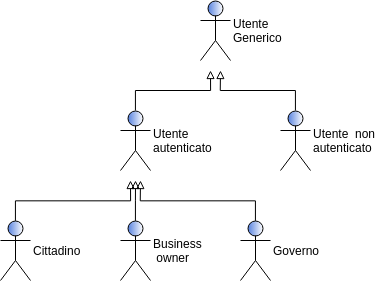
\includegraphics[width=7cm]{res/images/attori_primari.png}
	\centering
	\caption{Gerarchia attori primari}
\end{figure}
\begin{description}[style=nextline]
	\item[Utente Generico]
	Si riferisce ad un utente generico che accede alla piattaforma dal sito web;
	\item[Utente non autenticato]
	Si riferisce ad un utente generico che non ha ancora effettuato l'autenticazione alla piattaforma;
	\item[Utente autenticato]
	Si riferisce ad un utente generico che si è autenticato nel sistema con la procedura di login. Ciò implica che sia in possesso di una chiave pubblica valida sulla rete Ethereum con la quale, precedentemente, ha portato a termine la procedura di autenticazione;
	\item[Cittadino] Si riferisce ad un utente che si è autenticato nel sistema con il ruolo di cliente;
	\item[Azienda] Si riferisce ad un utente che si è autenticato nel sistema con il ruolo di azienda. Le azioni sono eseguite considerando l'azienda come persona giuridica, nonostante le azioni vengano eseguite da un suo rappresentante;
	\item[Governo\glo] Si riferisce ad un utente che si è autenticato al sistema con il ruolo di governo\glo.
\end{description}
\subsubsection{Attori secondari}\begin{description}[style=nextline]
	\item[MetaMask]
	Plug-in per browser che permette di interfacciarsi con la rete Ethereum\glosp e di validare le transazioni con la propria chiave privata.

\end{description}

\subsection{Elenco dei casi d'uso}
In questa sezione vi sono elencati tutti i casi d'uso individuati. Ogni caso d'uso rappresenta uno scenario per uno o più attori, ovviamente applicabile anche ad eventuali attori derivati. Un singolo caso d'uso inoltre viene esplicato tramite diagrammi dei casi d'uso e possiede una precondizione seguida da una postcondizione.
\begin{figure}[h]
	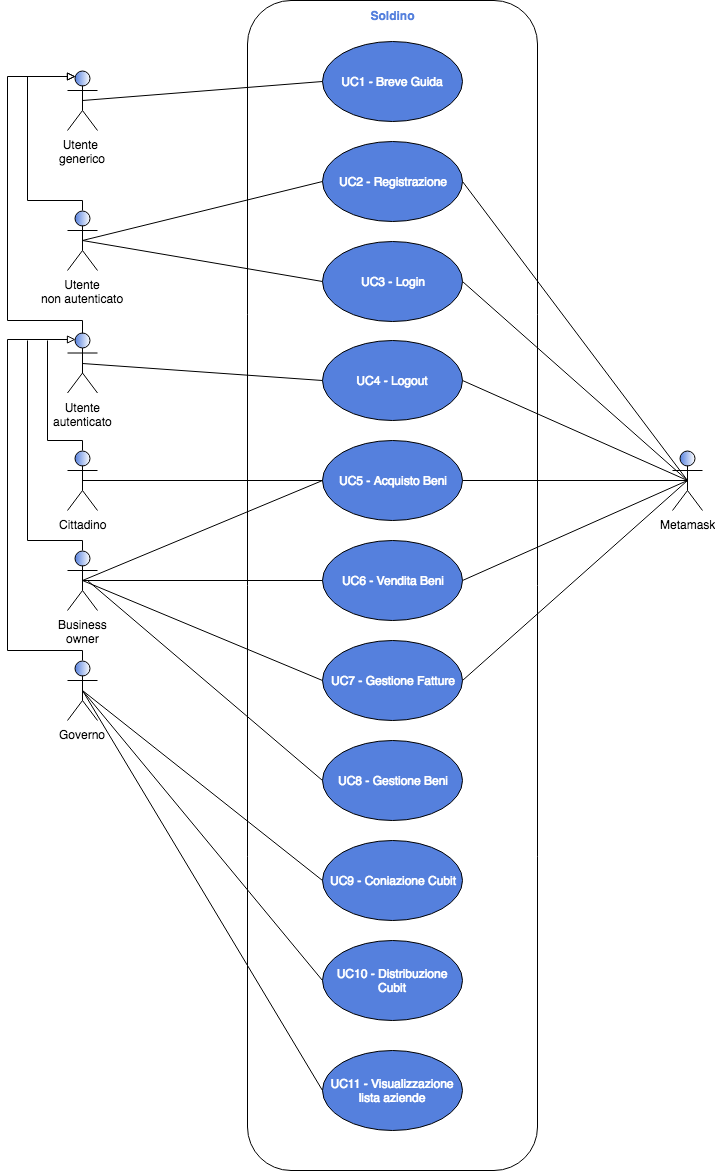
\includegraphics[width=9.38cm]{res/images/Elenco_casi_d_uso.png}
	\centering
	\caption{Elenco dei casi d'uso}
\end{figure}
\subsubsection{UC1 - Breve Guida}
\begin{itemize}
	\item \textbf{Attori Primari}
	\item \textbf{Descrizione}
	\item \textbf{Precondizione}
	\item \textbf{Postcondizione}
	\item \textbf{Scenario}
\end{itemize}
\subsubsection{UC2 - Registrazione}
\begin{itemize}
	\item \textbf{Attori Primari}
	\item \textbf{Descrizione}
	\item \textbf{Precondizione}
	\item \textbf{Postcondizione}
	\item \textbf{Scenario}
\end{itemize}
\subsubsection{UC3 - Login}
\begin{figure}[h]
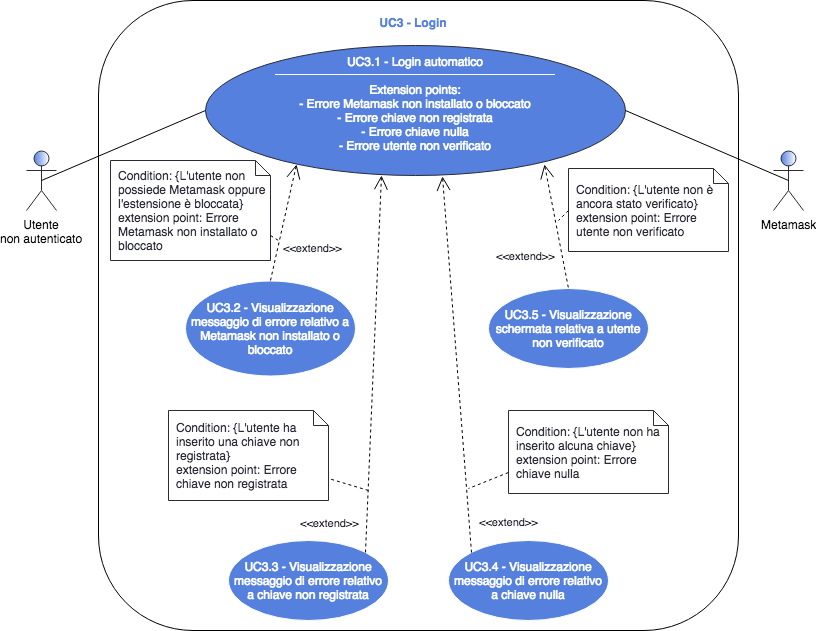
\includegraphics[width=14.5cm]{res/images/UC3Login.png}
\centering
\caption{UC3 - Login}

\end{figure}
\begin{itemize}
	\item \textbf{Attori Primari}
	Utente non autenticato
	\item \textbf{Attori Secondari}
	MetaMask\glo{}
	\item \textbf{Descrizione}
	L'utente prova a farsi identificare tramite l'interfaccia web per mezzo di MetaMask\glo{}.
	\item \textbf{Precondizione}
	L'utente non è identificato dalla piattaforma web.
	\item \textbf{Postcondizione}
	L'utente è identificato dalla piattaforma web. 
	\item \textbf{Scenario}
	L'utente non è identificato dal sito ed esegue il login.
\end{itemize}
\subsubsection{UC4 - Logout}
\begin{figure}[h]
	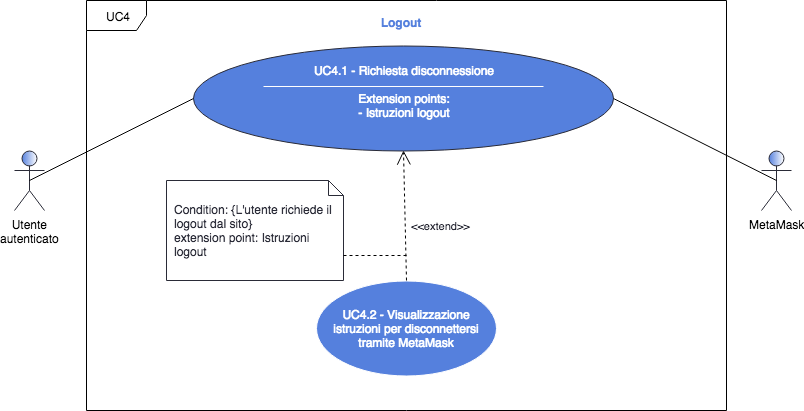
\includegraphics[width=14.5cm]{res/images/UC4Logout.png}
	\centering
	\caption{UC4 - Logout}
	
\end{figure}
\begin{itemize}
	\item \textbf{Attori Primari}
	Utente autenticato
	\item \textbf{Attori Secondari}
	MetaMask\glo{}
	\item \textbf{Descrizione}
	L'utente richiede il logout dalla piattaforma web ed effettua ciò tramite MetaMask\glo{}.
	\item \textbf{Precondizione}
	L'utente è identificato dalla piattaforma web e richiede di essere disconnesso dal sito.
	\item \textbf{Postcondizione}
	Vengono fornite le istruzioni necessarie per affrontare il Logout tramite MetaMask\glo{}. 
	\item \textbf{Scenario}
	L'utente è identificato dal sito ed esegue il logout.
\end{itemize}
\subsubsection{UC5 - Acquisto Beni}
\begin{itemize}
	\item \textbf{Attori Primari}
	\item \textbf{Descrizione}
	\item \textbf{Precondizione}
	\item \textbf{Postcondizione}
	\item \textbf{Scenario}
\end{itemize}
\subsubsection{UC6 - Vendita Beni}
\begin{itemize}
	\item \textbf{Attori Primari}
	\item \textbf{Descrizione}
	\item \textbf{Precondizione}
	\item \textbf{Postcondizione}
	\item \textbf{Scenario}
\end{itemize}
\subsubsection{UC7 - Gestione Fatture}
\begin{itemize}
	\item \textbf{Attori Primari}
	\item \textbf{Descrizione}
	\item \textbf{Precondizione}
	\item \textbf{Postcondizione}
	\item \textbf{Scenario}
\end{itemize}
\subsubsection{UC8 - Gestione Beni}
\begin{itemize}
	\item \textbf{Attori Primari}
	\item \textbf{Descrizione}
	\item \textbf{Precondizione}
	\item \textbf{Postcondizione}
	\item \textbf{Scenario}
\end{itemize}
\subsubsection{UC9 -  Coniazione Cubit}
\begin{itemize}
	\item \textbf{Attori Primari}
	\item \textbf{Descrizione}
	\item \textbf{Precondizione}
	\item \textbf{Postcondizione}
	\item \textbf{Scenario}
\end{itemize}
\subsubsection{UC10 - Distribuzione Cubit}
\begin{itemize}
	\item \textbf{Attori Primari}
	\item \textbf{Descrizione}
	\item \textbf{Precondizione}
	\item \textbf{Postcondizione}
	\item \textbf{Scenario}
\end{itemize}
\subsubsection{UC11 - Visualizzazione Lista Aziende}
\begin{itemize}
	\item \textbf{Attori Primari}
	\item \textbf{Descrizione}
	\item \textbf{Precondizione}
	\item \textbf{Postcondizione}
	\item \textbf{Scenario}
\end{itemize}


\pagebreak

\section{Requisiti} 
Ogni requisito è composto dalla seguente struttura:
\begin{itemize}
	\item \textbf{codice identificativo}: ogni codice identificativo è univoco e conforme alla seguente codifica: \\
	\centerline{\textbf{R[Importanza][Tipologia][Codice]}} \\ \\
	Il significato delle cui voci è:
	\begin{itemize}
		\item \textbf{Importanza}: ogni requisito può assumere uno dei seguenti valori:
		\begin{itemize}
			\item \textit{1}: requisito obbligatorio: irrinunciabili per qualcuno degli stakeholder;
			\item \textit{2}: requisito desiderabile: non strettamente necessari ma  a valore aggiunto riconoscibile;
			\item \textit{3}: requisito opzionale: relativamente utili oppure contrattabili più avanti nel progetto;	
		\end{itemize}
		\item \textbf{Tipologia}: ogni requisito può assumere uno dei seguenti valori:
		\begin{itemize}
			\item \textit{F}: funzionale;
			\item \textit{Q}: prestazionale;
			\item \textit{P}: qualitativo;
			\item \textit{V}: vincolo.
		\end{itemize}
		\item \textbf{Codice}: è un identificatore univoco del requisito in forma gerarchica padre/figlio.
	\end{itemize}
	\item \textbf{classificazione}: viene riportata l'importanza del requisito. Sebbene questa sia un'informazione ridondante ne facilita la lettura;
	\item \textbf{descrizione}: descrizione breve ma completa del requisito, meno ambigua possibile;
	\item \textbf{fonti}: ogni requisito può derivare da una o più tra le seguenti opzioni:
	\begin{itemize}
		\item \textit{capitolato\glo}: si tratta di un requisito individuato dalla lettura del capitolato\glo;
		\item \textit{interno}: si tratta di un requisito che gli analisti hanno ritenuto opportuno aggiungere;
		\item \textit{caso d'uso}: il requisito è estrapolato da uno o più casi d'uso. In questo caso è riportato il codice univoco del caso d'uso;
		\item \textit{verbale}: si tratta di un requisito individuato in seguito ad una richiesta di chiarimento con il proponente. Tali informazioni sono riportate nei verbali in cui ogni requisito individuato è segnato da un codice presente nella tabella dei tracciamenti.
	\end{itemize}
\end{itemize}
\renewcommand{\arraystretch}{1.5}

\subsection{Requisiti funzionali}

	\rowcolors{2}{pari}{dispari}
	
	\begin{longtable}{ >{\centering}p{0.15\textwidth} >{\centering}p{0.20\textwidth}
			>{\raggedright}p{0.35\textwidth} >{\centering}p{0.14\textwidth}}
		\caption{Tabella dei requisiti funzionali}\\
		\rowcolorhead 
		\textbf{\color{white}Requisito} 
		& \textbf{\color{white}Classificazione} 
		& \centering\textbf{\color{white}Descrizione}
		& \textbf{\color{white}Fonti} 
			\endfirsthead
		\rowcolor{white}\caption[]{(continua)}\\
		\rowcolorhead 
		\textbf{\color{white}Requisito} 
		& \textbf{\color{white}Classificazione} 
		& \centering\textbf{\color{white}Descrizione}
		& \textbf{\color{white}Fonti} 
		\endhead	
		
R2F1	&	Desiderabile	&	L’utente può leggere una breve guida sull’uso di MetaMask e sul pagamento delle operazioni	&	Interno\\ UC1	\tabularnewline
R1F2	&	Obbligatorio	&	Un utente non registrato può effettuare la registrazione	&	Capitolato	\tabularnewline
R1F2.1	&	Obbligatorio	&	Il sistema permette la registrazione di un nuovo cittadino	&	Capitolato	\tabularnewline
R1F2.1.1	&	Obbligatorio	&	La registrazione da parte di un cittadino necessita di email	&	Interno \\ UC2.2.1	\tabularnewline
R1F2.1.2	&	Obbligatorio	&	La registrazione da parte di un cittadino necessita di indirizzo	&	Interno \\ UC2.2.2	\tabularnewline
R1F2.1.3	&	Obbligatorio	&	La registrazione da parte di un cittadino necessita di una password	&	Interno \\ UC2.2.3	\tabularnewline
R1F2.1.4	&	Obbligatorio	&	La registrazione da parte di un cittadino necessita di nome	&	Interno \\ UC2.3.1	\tabularnewline
R1F2.1.5	&	Obbligatorio	&	La registrazione da parte di un cittadino necessita di cognome	&	Interno \\ UC2.3.2	\tabularnewline
R1F2.2	&	Obbligatorio	&	Il sistema permette la registrazione di una nuova azienda	&	Capitolato	\tabularnewline
R1F2.2.1	&	Obbligatorio	&	La registrazione da parte di un'azienda necessita di email	&	Interno \\ UC2.2.1	\tabularnewline
R1F2.2.2	&	Obbligatorio	&	La registrazione da parte di un'azienda necessita della sede	&	Interno \\ UC2.2.2	\tabularnewline
R1F2.2.3	&	Obbligatorio	&	La registrazione da parte di u'azienda necessita di una password	&	Interno \\ UC2.2.3	\tabularnewline
R1F2.2.4	&	Obbligatorio	&	La registrazione da parte di un'azienda necessita di partita IVA	&	Interno \\ UC2.4.1	\tabularnewline
R1F2.2.5	&	Obbligatorio	&	La registrazione da parte di un'azienda necessita di nome azienda	&	Interno \\ UC2.4.2	\tabularnewline
R1F2.3	&	Obbligatorio	&	La fase di registrazione di un nuovo utente non va a buon fine se la chiave è già presente nel sistema	&	Interno \\ UC2.7	\tabularnewline
R1F2.4	&	Obbligatorio	&	Il processo di registrazione di un nuovo utente si interrompe se almeno un campo non è stato compilato	&	Interno \\ UC2.9	\tabularnewline
R1F3	&	Obbligatorio	&	Un utente può effettuare il login	&	Interno \\ UC3	\tabularnewline
R1F3.1	&	Obbligatorio	&	Il login sulla piattaforma deve avvenire in modo automatico attraverso MetaMask	&	Capitolato\\ UC3.1	\tabularnewline
R1F3.2	&	Obbligatorio	&	Il processo di login e/o registrazione dell'utente non va a buon fine se MetaMask non è presente	&	Interno \\ UC2.5	\tabularnewline
R1F3.3	&	Obbligatorio	&	Il processo di login e/o registrazione dell'utente non va a buon fine se non vi è alcuna chiave disponibile nel plug-in	&	Interno \\ UC2.6	\tabularnewline
R1F3.4	&	Obbligatorio	&	Il processo di login si interrompe se la chiave inserita non è registrata nel sistema	&	Interno \\ UC3.2	\tabularnewline
R1F3.5	&	Obbligatorio	&	Il processo di login e/o registrazione dell'utente non va a buon fine se l'utente risulta "disabilitato"	&	Interno \\ UC3.3	\tabularnewline
R1F4	&	Obbligatorio	&	L'utente può effettuare il logout	&	Interno\\ UC4	\tabularnewline
R1F5	&	Obbligatorio	&	Il governo può coniare Cubit	&	Capitolato \\ UC9	\tabularnewline
R1F5.1	&	Obbligatorio	&	Il governo può inserire la quantità di Cubit da coniare	&	Interno \\ UC9	\tabularnewline
R1F6	&	Obbligatorio	&	Il governo può distribuire Cubit a cittadini ed aziende	&	Capitolato \\ UC10	\tabularnewline
R1F6.1	&	Obbligatorio	&	Il governo può determinare l’ammontare di Cubit pro capite da trasferire	&	Interno\\ UC10.1	\tabularnewline
R1F6.2	&	Obbligatorio	&	Il governo può selezionare la lista dei destinatari del trasferimento dalla lista degli utenti	&	Interno\\ UC10.2	\tabularnewline
R1F6.3	&	Obbligatorio	&	La distribuzione dei Cubit da parte del governo fallisce mostrando un errore se è stata raggiunta la soglia massima distribuibile	&	Interno\\ UC10.4	\tabularnewline
R1F7	&	Obbligatorio	&	Il governo può visualizzare e gestire la lista degli utenti registrati	&	Interno \\ UC11	\tabularnewline
R1F7.1	&	Obbligatorio	&	Il governo può visualizzare lo stato di "abilitato" o "disabilitato" per un utente registrato	&	Interno \\ UC11.1	\tabularnewline
R1F7.1.1	&	Obbligatorio	&	Il governo può disabilitare l'account di un utente registrato	&	Interno \\ UC12.2	\tabularnewline
R3F7.1.1.1	&	Opzionale	&	Il governo può motivare con un messaggio la scelta di disabilitazione di un account	&	Interno \\ UC12.3	\tabularnewline
R1F7.1.2	&	Obbligatorio	&	Il governo può abilitare l'account, precedentemente disabilitato, di un utente registrato	&	Interno \\ UC12.1	\tabularnewline
R1F7.2	&	Obbligatorio	&	Il governo può visualizzare e gestire la lista delle aziende registrate	&	Capitolato \\ UC11.1	\tabularnewline
R1F7.2.1	&	Obbligatorio	&	Il governo può visualizzare la chiave Ethereum di ogni azienda	&	Interno \\ UC11.1	\tabularnewline
R1F7.2.2	&	Obbligatorio	&	Il governo può visualizzare il nome di ogni azienda	&	Interno \\ UC11.1	\tabularnewline
R1F7.2.3	&	Obbligatorio	&	Il governo può visualizzare la partita IVA di ogni azienda	&	Interno \\ UC11.1	\tabularnewline
R1F7.2.4	&	Obbligatorio	&	Il governo può visualizzare la sede di ogni azienda	&	Interno \\ UC11.1	\tabularnewline
R1F7.2.5	&	Obbligatorio	&	Il governo può visualizzare lo stato del pagamento del saldo IVA e relativo importo di ogni azienda	&	Interno \\ UC11.1	\tabularnewline
R1F7.2.6	&	Obbligatorio	&	Il governo può visualizzare la lista delle aziende filtrando i risultati per il valore \texttt{stato di liquidazione IVA}, che può assumere i valori: insolvente,  in fase di pagamento, in dilazione,  regolare, in attesa di rimborso	&	Interno \\ UC11.1.1	\tabularnewline
R1F7.2.7	&	Obbligatorio	&	Il governo può effettuare il rimborso alle aziende il cui stato di liquidazione IVA risulta in attesa di rimborso	&	Interno  \\ UC13	\tabularnewline
R1F7.2.7.1	&	Obbligatorio	&	Un errore viene visualizzato nel caso in cui il governo tenti di effettuare il rimboroso IVA ma i fondi non sono suficienti ad eseguire quest'operazione	&	Interno \\ UC7.5	\tabularnewline
R1F7.3	&	Obbligatorio	&	Il governo può visualizzare e gestire la lista dei cittadini registrati	&	Interno \\ UC11.2	\tabularnewline
R1F7.3.1	&	Obbligatorio	&	Il governo può visualizzare la chiave\glosp di ogni cittadino	&	Interno \\ UC11.2	\tabularnewline
R1F7.3.2	&	Obbligatorio	&	Il governo può visualizzare il nome di ogni cittadino	&	Interno \\ UC11.2	\tabularnewline
R1F7.3.3	&	Obbligatorio	&	Il governo può visualizzare il cognome di ogni cittadino	&	Interno\\ UC11.2	\tabularnewline
R1F7.3.4	&	Obbligatorio	&	Il governo può visualizzare l'indirizzo di ogni cittadino	&	Interno\\ UC11.2	\tabularnewline
R1F7.3.5	&	Obbligatorio	&	Il governo può visualizzare l'email di ogni cittadino	&	Interno\\ UC11.2	\tabularnewline
R1F8	&	Obbligatorio	&	Aziende e cittadini possono visualizzare i prodotti in vendita nel sito	&	Interno\\ UC5	\tabularnewline
R1F8.1	&	Obbligatorio	&	Aziende e cittadini possono visualizzare il nome di ciascun prodotto in vendita nel sito	&	Interno\\ UC5	\tabularnewline
R1F8.2	&	Obbligatorio	&	Aziende e cittadini possono visualizzare il prezzo lordo di ciascun prodotto in vendita nel sito	&	Interno\\ UC5	\tabularnewline
R1F8.3	&	Obbligatorio	&	Aziende e cittadini possono visualizzare la descrizione di ciascun prodotto in vendita nel sito	&	Interno\\ UC5	\tabularnewline
R1F8.4	&	Obbligatorio	&	Aziende e cittadini possono visualizzare la quantità di prodotto selezionato relativa a ciascun prodotto in vendita nel sito	&	Interno\\ UC5	\tabularnewline
R1F8.4.1	&	Obbligatorio	&	Aziende e cittadini possono modificare la quantità di prodotto selezionata relativa a ciascun prodotto in vendita nel sito	&	Interno\\ UC5.1	\tabularnewline
R1F9	&	Obbligatorio	&	Aziende e cittadini possono aggiungere prodotti al carrello	&	Interno\\ UC6.1	\tabularnewline
R1F10	&	Obbligatorio	&	Aziende e cittadini possono visualizzare i prodotti nel carrello	&	Interno\\ UC6.2	\tabularnewline
R1F10.1	&	Obbligatorio	&	Aziende e cittadini possono visualizzare il nome di ciascun prodotto nel carrello	&	Interno\\ UC6.2	\tabularnewline
R1F10.2	&	Obbligatorio	&	Aziende e cittadini possono visualizzare la quantità di ciascun prodotto nel carrello	&	Interno\\ UC6.2	\tabularnewline
R1F10.3	&	Obbligatorio	&	Aziende e cittadini possono visualizzare il prezzo unitario di ciascun prodotto nel carrello	&	Interno\\ UC6.2	\tabularnewline
R1F10.4	&	Obbligatorio	&	Aziende e cittadini possono visualizzare il prezzo totale dei prodotti nel carrello	&	Interno\\ UC6.2	\tabularnewline
R1F11	&	Obbligatorio	&	Aziende e cittadini possono modificare la quantità di un bene da acquistare presente nel carrello	&	Interno \\UC6.3	\tabularnewline
R1F12	&	Obbligatorio	&	Aziende e cittadini possono rimuovere prodotti dal carrello	&	Interno\\ UC6.4	\tabularnewline
R1F13	&	Obbligatorio	&	Il sistema di compravendita deve essere implementato secondo il meccanismo di escrow\glo	&	Interno	\tabularnewline
R1F14	&	Obbligatorio	&	Aziende e cittadini posso acquistare prodotti venduti nella piattaforma	&	Capitolato\\ UC7	\tabularnewline
R1F14.1	&	Obbligatorio	&	Aziende e cittadini possono effettuare il checkout dei prodotti contenuti nel carrello	&	Interno\\ UC7.1	\tabularnewline
R1F14.1.1	&	Obbligatorio	&	In fase di checkout viene visualizzato un messaggio di errore se il carrello è vuoto	&	Interno\\ UC7.2	\tabularnewline
R1F14.2	&	Obbligatorio	&	La fase di acquisto necessita di un indirizzo di spedizione	&	Interno\\ UC7.3	\tabularnewline
R1F14.2.1	&	Obbligatorio	&	L'acquirente può selezionare come indirizzo di spedizione il proprio indirizzo di residenza	&	Interno\\ UC7.3	\tabularnewline
R1F14.2.2	&	Obbligatorio	&	L'acquirente può inserire un nuovo indirizzo per la spedizione	&	Interno\\ UC7.3	\tabularnewline
R1F14.3	&	Obbligatorio	&	Viene visualizzato un messaggio di errore se il pagamento non va a buon fine	&	Interno\\ UC7.5	\tabularnewline
R1F14.4	&	Obbligatorio	&	Il sistema genera la conferma d'ordine\glo, che viene visualizzata nella pagina dedicata dell'acquirente (meccanismo di escrow\glo)	&	Interno	\tabularnewline
R1F14.5	&	Obbligatorio	&	Il sistema trattiene l'ammontare del pagamento fino all'approvazione/rifiuto della conferma d'ordine\glosp (meccanismo di escrow\glo)	&	Interno	\tabularnewline
R1F15	&	Obbligatorio	&	Aziende e cittadini  possono visualizzare la lista degli acquisti effettuati	&	Interno\\ UC14.1	\tabularnewline
R1F15.1	&	Obbligatorio	&	Il riepilogo di un acquisto effettuato include la data dell'acquisto	&	Interno\\ UC14.1	\tabularnewline
R1F15.2	&	Obbligatorio	&	Il riepilogo di un acquisto effettuato include il numero dell'acquisto	&	Interno\\ UC14.1	\tabularnewline
R1F15.3	&	Obbligatorio	&	Il riepilogo di un acquisto effettuato include i prodotti includi nell'acquisto	&	Interno\\ UC14.1	\tabularnewline
R1F15.4	&	Obbligatorio	&	Il riepilogo di un acquisto effettuato include il totale IVA dell'acquisto	&	Interno\\ UC14.1	\tabularnewline
R1F15.5	&	Obbligatorio	&	Il riepilogo di un acquisto effettuato include il  prezzo lordo dell'acquisto	&	Interno\\ UC14.1	\tabularnewline
R1F15.6	&	Obbligatorio	&	Il riepilogo di un acquisto effettuato include l'indirizzo di spedizione dell'acquisto	&	Interno\\ UC14.1	\tabularnewline
R1F15.7	&	Obbligatorio	&	Aziende e cittadini possono visualizzare le conferme d'ordine da approvare	&	Interno \\ UC14.2	\tabularnewline
R1F15.7.1	&	Obbligatorio	&	Aziende e cittadini possono rifiutare le conferme d'ordine in attesa di approvazione	&	Interno \\ UC14.5	\tabularnewline
R1F15.7.1.1	&	Obbligatorio	&	La somma totale dell'ordine rifutato viene rimborsata all'acquirente	&	Interno \\ UC14.4	\tabularnewline
R2F15.7.1.2	&	Desiderabile	&	Aziende e cittadini possono annullare un'ordine d'acquisto entro 2 giorni dal ricevimento dello stesso	&	Interno	\tabularnewline
R1F15.7.2	&	Obbligatorio	&	Aziende e cittadini possono approvare le conferme d'ordine in attesa di approvazione	&	Interno \\ UC14.6	\tabularnewline
R2F15.8	&	Desiderabile	&	Aziende e cittadini ricevono notifiche via email con aggiornamenti sull'ordine	&	Interno	\tabularnewline
R1F16	&	Obbligatorio	&	Un'azienda può gestire i prodotti in vendita	&	Capitolato\\ UC8	\tabularnewline
R1F16.1	&	Obbligatorio	&	Un'azienda può mettere in vendita beni e servizi	&	Capitolato\\ UC8.1	\tabularnewline
R1F16.1.1	&	Obbligatorio	&	I nuovi prodotti devono indicare il prezzo netto di vendita	&	Interno\\ UC8.1.3	\tabularnewline
R1F16.1.2	&	Obbligatorio	&	I nuovi prodotti devono avere una descrizione	&	Interno\\ UC8.1.2	\tabularnewline
R1F16.1.3	&	Obbligatorio	&	I nuovi prodotti devono indicare l'aliquota IVA	&	Interno\\ UC8.1.4	\tabularnewline
R1F16.1.4	&	Obbligatorio	&	I nuovi prodotti devono avere un nome	&	Interno\\ UC8.1.1	\tabularnewline
R1F16.1.5	&	Obbligatorio	&	Durante l'inserimento di un prodotto, il processo fallisce se almeno un campo non è stato compilato	&	Interno\\ UC2.9	\tabularnewline
R1F16.2	&	Obbligatorio	&	Un'azienda può modificare i dati relativi ad un proprio bene o servizio in vendita	&	Capitolato\\ UC8.3	\tabularnewline
R1F16.2.1	&	Obbligatorio	&	Durante la modifica di un prodotto, il processo fallisce se non è stato modificato alcun campo	&	Interno\\ UC8.3.6	\tabularnewline
R1F16.3	&	Obbligatorio	&	Un'azienda può eliminare un proprio bene o servizio in vendita	&	Capitolato\\ UC8.4	\tabularnewline
R1F17	&	Obbligatorio	&	Un'azienda può visualizzare la lista delle vendite 	&	Interno\\ UC14.3	\tabularnewline
R1F17.1	&	Obbligatorio	&	Il riepilogo di una vendita effettuata include la data della vendita	&	Interno\\ UC14.1	\tabularnewline
R1F17.2	&	Obbligatorio	&	Il riepilogo di una vendita effettuata include il numero della vendita	&	Interno\\ UC14.1	\tabularnewline
R1F17.3	&	Obbligatorio	&	Il riepilogo di una vendita effettuata include i prodotti includi della vendita	&	Interno\\ UC14.1	\tabularnewline
R1F17.4	&	Obbligatorio	&	Il riepilogo di una vendita effettuata include il totale IVA della vendita	&	Interno\\ UC14.1	\tabularnewline
R1F17.5	&	Obbligatorio	&	Il riepilogo di una vendita effettuata include il prezzo lordo della vendita	&	Interno\\ UC14.1	\tabularnewline
R1F17.6	&	Obbligatorio	&	Il riepilogo di una vendita effettuata include l'indirizzo di spedizione della vendita	&	Interno\\ UC14.1	\tabularnewline
R1F17.7	&	Obbligatorio	&	Il riepilogo di una vendita effettuata include la data di approvazione dell'acquisto	&	Interno\\ UC14.3	\tabularnewline
R1F17.8	&	Obbligatorio	&	Il riepilogo di una vendita effettuata include il nome dell'acquirente se esso è un cittadino	&	Interno\\ UC14.3	\tabularnewline
R1F17.9	&	Obbligatorio	&	Il riepilogo di una vendita effettuata include il cognome dell'acquirente se esso è un cittadino	&	Interno\\ UC14.3	\tabularnewline
R1F17.10	&	Obbligatorio	&	Il riepilogo di una vendita effettuata include il nome dell'azienda-cliente se essa è l'acquirente	&	Interno\\ UC14.3	\tabularnewline
R1F17.11	&	Obbligatorio	&	Il riepilogo di una vendita effettuata include la partita IVA dell'azienda-cliente se essa è l'acquirente	&	Interno\\ UC14.3	\tabularnewline
R1F18	&	Obbligatorio	&	Un'azienda riceve il pagamento a seguito della conferma d'ordine da parte di un acquirente (meccanismo di escrow\glo)	&	Interno \\ UC14.5	\tabularnewline
R1F19	&	Obbligatorio	&	Un'azienda può gestire le transazioni riguardanti l'IVA	&	Capitolato \\ UC15	\tabularnewline
R1F19.1	&	Obbligatorio	&	Un'azienda può visualizzare il saldo IVA relativo al trimestre corrente	&	Interno \\ UC15.3	\tabularnewline
R1F19.2	&	Obbligatorio	&	Un'azienda può visualizzare il saldo IVA relativo ad un trimestre concluso selezionato	&	Interno \\ UC15.4	\tabularnewline
R1F19.3	&	Obbligatorio	&	Un'azienda può visualizzare per ogni saldo IVA la lista delle fatture relative al trimestre selezionato(vista generale delle fatture) ed il valore del saldo stesso	&	Interno \\ UC15.2	\tabularnewline
R1F19.3.1	&	Obbligatorio	&	La vista generale della fattura include il numero identificativo della fattura	&	Interno \\ UC15.2	\tabularnewline
R1F19.3.2	&	Obbligatorio	&	La vista generale della fattura include la data della fattura	&	Interno \\ UC15.2	\tabularnewline
R1F19.3.3	&	Obbligatorio	&	La vista generale della fattura include il nome dell'azienda emittente (inteso come ragione sociale)	&	Interno \\ UC15.2	\tabularnewline
R1F19.3.4	&	Obbligatorio	&	La vista generale della fattura include informazioni relative all'acquirente	&	Interno \\ UC15.2	\tabularnewline
R1F19.3.4.1	&	Obbligatorio	&	La vista generale della fattura include nome e cognome dell'acquirente nel caso questo sia un cittadino	&	Interno \\ UC15.2	\tabularnewline
R1F19.3.4.2	&	Obbligatorio	&	La vista generale della fattura include nome dell'azienda acquirente nel caso sia appunto un'azienda 	&	Interno \\ UC15.2	\tabularnewline
R1F19.3.5	&	Obbligatorio	&	La vista generale della fattura include l'importo totale dell'ordine	&	Interno \\ UC15.2	\tabularnewline
R1F19.3.6	&	Obbligatorio	&	La vista generale della fattura include l'IVA a credito/debito derivato dalla transazione	&	Interno \\ UC15.2	\tabularnewline
R1F19.4	&	Obbligatorio	&	Un'azienda può effettuare il versamento IVA di un trimestre nel quale il saldo IVA risulti a debito	&	Capitolato \\ UC15.6	\tabularnewline
R1F19.5	&	Obbligatorio	&	Un'azienda può effettuare la dilazione del versamento IVA di un trimestre nel quale il saldo IVA risulti a debito	&	Capitolato \\ UC15.7	\tabularnewline
R1F19.6	&	Obbligatorio	&	Un'azienda può scaricare in formato PDF la lista dei movimenti IVA per l'attuale trimestre	&	Capitolato\\ UC15.5	\tabularnewline
R1F19.7	&	Obbligatorio	&	Un'azienda può visualizzare in dettaglio una particolare fattura 	&	Interno\\ UC15.8	\tabularnewline
R1F19.7.1	&	Obbligatorio	&	La fattura include la data della fattura	&	Interno\\ UC15.8	\tabularnewline
R1F19.7.2	&	Obbligatorio	&	La fattura include il numero identificativo della fattura	&	Interno\\ UC15.8	\tabularnewline
R1F19.7.3	&	Obbligatorio	&	La fattura include la data dell'ordine relativo alla fattura	&	Interno\\ UC15.8	\tabularnewline
R1F19.7.4	&	Obbligatorio	&	La fattura include il numero identificativo dell'ordine relativo alla fattura	&	Interno\\ UC15.8	\tabularnewline
R1F19.7.5	&	Obbligatorio	&	La fattura include la visualizzazione dei prodotti 	&	Interno\\ UC15.8	\tabularnewline
R1F19.7.5.1	&	Obbligatorio	&	Per ogni prodotto elencato in una fattura è visualizzato il nome	&	Interno\\ UC15.8	\tabularnewline
R1F19.7.5.2	&	Obbligatorio	&	Per ogni prodotto elencato in una fattura è visualizzata la descizione	&	Interno\\ UC15.8	\tabularnewline
R1F19.7.5.3	&	Obbligatorio	&	Per ogni prodotto elencato in una fattura è visualizzata la quantità	&	Interno\\ UC15.8	\tabularnewline
R1F19.7.5.4	&	Obbligatorio	&	Per ogni prodotto elencato in una fattura è visualizzato il prezzo netto	&	Interno\\ UC15.8	\tabularnewline
R1F19.7.5.5	&	Obbligatorio	&	Per ogni prodotto elencato in una fattura è visualizzata l'aliquota IVA	&	Interno\\ UC15.8	\tabularnewline
R1F19.7.5.6	&	Obbligatorio	&	Per ogni prodotto elencato in una fattura è visualizzato il prezzo lordo	&	Interno\\ UC15.8	\tabularnewline
R1F19.7.6	&	Obbligatorio	&	La fattura include l'importo totale IVA della fattura	&	Interno\\ UC15.8	\tabularnewline
R1F19.7.7	&	Obbligatorio	&	La fattura include l'importo totale della fattura	&	Interno\\ UC15.8	\tabularnewline
R1F19.7.8	&	Obbligatorio	&	La fattura include il nome dell'azienda emittente	&	Interno\\ UC15.8	\tabularnewline
R1F19.7.9	&	Obbligatorio	&	La fattura include la partita IVA dell'azienda emittente	&	Interno\\ UC15.8	\tabularnewline
R1F19.7.10	&	Obbligatorio	&	La fattura include il nome dell'acquirente se esso è un cittadino	&	Interno\\ UC15.8	\tabularnewline
R1F19.7.11	&	Obbligatorio	&	La fattura include il cognome dell'acquirente se esso è un cittadino	&	Interno\\ UC15.8	\tabularnewline
R1F19.7.12	&	Obbligatorio	&	La fattura include il nome dell'azienda-cliente se essa è l'acquirente	&	Interno\\ UC15.8	\tabularnewline
R1F19.7.13	&	Obbligatorio	&	La fattura include la partita IVA dell'azienda-cliente se essa è l'acquirente	&	Interno\\ UC15.8	\tabularnewline
R1F19.7.14	&	Obbligatorio	&	La fattura include l'indirizzo di spedizione dell'ordine	&	Interno\\ UC15.8	\tabularnewline
R1F19.8	&	Obbligatorio	&	Un'azienda può scaricare in formato PDF la lista dei movimenti IVA per un trimestre selezionato	&	Capitolato\\ Interno	\tabularnewline
R3F19.9	&	Opzionale	&	L'azienda può scaricare in formato PDF la fattura relativa ad un acquisto	&	Interno	\tabularnewline
		
		
		
		
	\end{longtable}


\pagebreak
\subsection{Requisiti di qualità}

\rowcolors{2}{pari}{dispari}
\LTcapwidth=\linewidth
\begin{longtable}{ >{\centering}p{0.10\textwidth} >{\centering}p{0.25\textwidth}
		>{\raggedright}p{0.35\textwidth} >{\centering}p{0.14\textwidth}}
	\caption{Tabella dei requisiti di qualità}\\
	\rowcolorhead 
	\textbf{\color{white}Requisito} 
	& \textbf{\color{white}Classificazione} 
	& \centering\textbf{\color{white}Descrizione}
	& \textbf{\color{white}Fonti} 
	\endfirsthead
	\rowcolor{white}\caption{(continua)}\\
	\rowcolorhead 
	\textbf{\color{white}Requisito} 
	& \textbf{\color{white}Classificazione} 
	& \centering\textbf{\color{white}Descrizione}
	& \textbf{\color{white}Fonti} 
	\endhead
	R1Q1	&	Obbligatorio	&	La progettazione e la codifica devono rispettare le norme e le metriche definite nel documento \textit{Piano di qualifica v1.0.0}	&	Interno	\tabularnewline
	R1Q2	&	Obbligatorio	&	L’approccio di scrittura per il codice JavaScript deve rispettare il promise centric approach	&	Capitolato	\tabularnewline
	R1Q2.1	&	Obbligatorio	&	L'utilizzo delle callback\glosp deve essere possibilmente evitato, utilizzato solo se strettamente necessario	&	Capitolato	\tabularnewline
	R1Q3	&	Obbligatorio	&	La guida sullo stile di programmazione Airbnb JavaScript style guide deve essere rispettata nella stesura del codice JavaScript	&	Capitolato	\tabularnewline
	R1Q4	&	Obbligatorio	&	Lo sviluppo del codice JavaScript deve essere supportato dal software di analisi del codice ESLint\glo	&	Capitolato	\tabularnewline
	R1Q5	&	Obbligatorio	&	Il codice deve essere reso pubblico e versionato in una repositoty\glosp ospitata in un sistema di versionamento a scelta fra GitHub o GitLab	&	Capitolato	\tabularnewline
	R1Q6	&	Obbligatorio	&	La documentazione per l'utilizzo del software deve essere stesa in lingua inglese	&	Verbale 2018-12-07, VE\_1.5	\tabularnewline
	R1Q6.1	&	Obbligatorio	&	Il codice deve essere accompagnato da un manuale amministratore, che conterrà le informazioni per la distribuzione ed installazione dei software necessari	&	Capitolato	\tabularnewline
	R1Q6.2	&	Obbligatorio	&	Il codice deve essere accompagnato da un manuale utente, che esplicherà l'utilizzo dell'applicativo ad aziende, cittadini ed utenti governativi	&	Capitolato	\tabularnewline

	
\end{longtable}
	


\subsection{Requisiti di vincolo}

	\rowcolors{2}{pari}{dispari}
	
	\begin{longtable}{ >{\centering}p{0.10\textwidth} >{\centering}p{0.25\textwidth}
			>{\raggedright}p{0.35\textwidth} >{\centering}p{0.14\textwidth}}
		\caption{Tabella dei requisiti di vincolo}\\
		\rowcolorhead 
		\textbf{\color{white}Requisito} 
		& \textbf{\color{white}Classificazione} 
		& \centering\textbf{\color{white}Descrizione}
		& \textbf{\color{white}Fonti} 
			\endfirsthead
		\rowcolor{white}\caption[]{(continua)}\\
		\rowcolorhead 
		\textbf{\color{white}Requisito} 
		& \textbf{\color{white}Classificazione} 
		& \centering\textbf{\color{white}Descrizione}
		& \textbf{\color{white}Fonti} 
		\endhead	
		
		
R1V1	&	Obbligatorio	&	La Dapp\glosp sviluppata deve avere il front end\glosp sviluppato attraverso l'uso di tecnologie web	&	Capitolato	\tabularnewline
R1V1.1	&	Obbligatorio	&	L'applicativo deve essere sviluppato utilizzando JavaScript 8 (ES8)	&	Capitolato	\tabularnewline
R1V1.2	&	Obbligatorio	&	L'applicativo deve essere sviluppato utilizzando React\glo.	&	Capitolato	\tabularnewline
R1V1.3	&	Obbligatorio	&	L'applicativo deve essere sviluppato utilizzando Redux\glo.	&	Capitolato	\tabularnewline
R3V1.4	&	Opzionale	&	L'applicativo deve essere implementato affidandosi al boilerplate\glosp Gigacore\glo.	&	Capitolato	\tabularnewline
R2V1.5	&	Desiderabile	&	È desiderabile che l'applicativo venga sviluppato utilizzando SCSS\glo/Sass\glo	&	Capitolato	\tabularnewline
R1V2	&	Obbligatorio	&	Soldino deve rispettare lo standard EIP-712\glo.	&	Capitolato	\tabularnewline
R1V3	&	Obbligatorio	&	Gli smart contracs\glosp devono essere scritti in linguaggio Solidity\glo	&	Capitolato	\tabularnewline
R1V4.1	&	Obbligatorio	&	Per connettersi alla rete Ethereum\glosp deve essere utilizzato il plug-in\glosp MetaMask\glo	&	Capitolato	\tabularnewline
R1V4.2	&	Obbligatorio	&	Per poter validare ed effettuare una transazione che richiede un trasferimento di Cubit\glo, deve essere utilizzato MetaMask\glo	&	Capitolato	\tabularnewline
R1V5	&	Obbligatorio	&	Il sistema, ed in particolare lo sviluppo degli smart contracts\glo, deve avvenire per mezzo del framework\glosp Truffle\glo	&	Capitolato	\tabularnewline
R1V6	&	Obbligatorio	&	Lo sviluppo dell'applicativo deve comprendere l'implementazione di test di unità e di intergrazione	&	Capitolato	\tabularnewline
R1V7	&	Obbligatorio	&	Il progetto deve utilizzare come minimo i seguenti ambienti di sviluppo: ambiente di sviluppo locale, ambiente per il testing, ambiente per lo staging\glosp e ambiente di produzione.	&	Capitolato	\tabularnewline
R2V7.1	&	Desiderabile	&	Gli ambienti per le fasi di sviluppo locale e testing possono essere fornite da Truffle\glo, utilizzando la rete \textit{testrpc}\glosp ed il web server fornito dal framework\glosp stesso	&	Capitolato	\tabularnewline
R1V7.2	&	Obbligatorio	&	Durante la fase di staging l'applicazione deve pubblicamente accessibile	&	Capitolato	\tabularnewline
R2V7.3	&	Desiderabile	&	Come ambiente per la fase di staging è desiderabile l'utilizzo della rete Ropsten\glosp e del web server Surge.sh\glo	&	Capitolato	\tabularnewline
R3V7.4	&	Opzionale	&	L'ambiente di produzione deve essere composto dall'Ethereum\glosp main network assieme al web server Surge.sh\glo	&	Capitolato	\tabularnewline
%R1V8 è stato portato nei requisiti funzionali -> R1F21
%R1V8	&	Obbligatorio	&	L'utente non può effettuare alcuna azione prima di essersi autenticato al sistema con MetaMask\glo	&	Capitolato	\tabularnewline
R1V9.1	&	Obbligatorio	&	La Dapp\glosp dovrà essere accessibile ed utilizzabile utilizzando i browser Google Chrome, dalla versione 71	&	Verbale 2018-12-07  VE\_1.4	\tabularnewline
R1V9.2	&	Obbligatorio	&	La Dapp\glosp dovrà essere accessibile ed utilizzabile utilizzando il browser Mozilla FireFox, dalla versione 64	&	Verbale 2018-12-07 VE\_1.5	\tabularnewline
R1V10	&	Obbligatorio	&	Il token\glosp utilizzato nella piattaforma, il Cubit\glo, dovrà rispettare lo standard ECR20\glo	&	Capitolato	\tabularnewline
R1V11	&	Obbligatorio	&	Il sistema deve essere pubblicato con licenza MIT	&	Capitolato	\tabularnewline
R1V12	&	Obbligatorio	&	Il sistema di compravendita deve essere implementato secondo il meccanismo di escrow\glo	&	Verbale 2019-01-04  VE\_3.4	\tabularnewline
R1V13	&	Obbligatorio	&	I pagamenti riguardanti i saldi IVA non devono avvenire automaticamente	&	Verbale 2018-12-07 VE\_1.2	\tabularnewline
R2V14	&	Desiderabile	&	Il codice deve essere versionato in una repositoty\glosp ospitata in un sistema di versionamento, ad esempio GitHub o GitLab	&	Capitolato	\tabularnewline
R1V15	&	Obbligatorio	&	La documentazione per l'utilizzo del software deve essere stesa in lingua inglese	&	Verbale 2018-12-07, VE\_1.6	\tabularnewline
R1V15.1	&	Obbligatorio	&	Il codice deve essere accompagnato da un manuale amministratore, che conterrà le informazioni per la distribuzione ed installazione dei software necessari	&	Capitolato	\tabularnewline
R1V15.2	&	Obbligatorio	&	Il codice deve essere accompagnato da un manuale utente, che esplicherà l'utilizzo dell'applicativo ad aziende, cittadini ed utenti governativi	&	Capitolato	\tabularnewline
R1V16	&	Opzionale	&	Sviluppare un metodo di pagamento veloce implementato con la rete Raiden\glo	&	Capitolato	\tabularnewline
		
		
		
		
	\end{longtable}


\subsection{Requisiti prestazionali}
Non sono stati individuati requisiti prestazionali in quanto il progetto sarà costituito da una ÐApp\glo, e come database di supporto verrà utilizzato un database distribuito. L'utilizzo di queste tecnologie prevede l'interazione con una rete Ethereum\glosp nel primo caso, e con una rete peer-to-peer\glosp nel secondo. Le operazioni che avvengono in una rete Ethereum\glosp reale hanno un tempo di soddisfacimento che dipende dal carico della rete nel momento della richiesta. Nel caso queste operazioni vadano a modificare un contratto, sarà inoltre il quantitativo di Ether per unità di Gas\glosp a determinarne la priorità di esecuzione all'interno della rete. Situazione simile per quanto riguarda il database distribuito, dove la velocità di reperimento delle informazioni dipende dal numero di peer attualmente disponibili.
\pagebreak
\subsection{Tracciamento}  
\subsubsection{Fonte - Requisiti}

	\rowcolors{2}{pari}{dispari}
	
	\begin{longtable}{ >{\centering}p{0.5\textwidth}
			>{\centering}p{0.5\textwidth}}
		\caption{Tabella di tracciamento fonte-requisiti}\\
		\rowcolorhead 
		\textbf{\color{white}Fonte}
		& \textbf{\color{white}Requisiti} 
		\tabularnewline 	
		\endfirsthead
		\rowcolor{white}\caption[]{(continua)} \\
		\rowcolorhead 
		\textbf{\color{white}Fonte}
		& \textbf{\color{white}Requisiti} 
		\tabularnewline 
		\endhead
		
	Capitolato	&	R1F2\\ 
	R1F2.1\\ 
	R1F2.2\\ 
	R1F3.1\\ 
	R1F5\\ 
	R1F6\\ 
	R1F7.2\\ 
	R1F14\\ 
	R1F16\\ 
	R1F16.1\\ 
	R1F16.2\\ 
	R1F16.3\\ 
	R1F19\\ 
	R1F19.4\\ 
	R1F19.6\\ 
	R1F19.8\\ 
	R1Q2\\ 
	R1Q2.1\\ 
	R1Q3\\ 
	R1Q4\\ 
	R1V1\\ 
	R1V1.1\\ 
	R1V1.2\\ 
	R1V1.3\\ 
	R3V1.4\\ 
	R2V1.5\\ 
	R1V2\\ 
	R1V3.1\\ 
	R1V3.2\\
	R1V4.1\\ 
	R1V4.2\\ 
	R1V5\\ 
	R1V6\\ 
	R1V7\\ 
	R2V7.1\\ 
	R1V7.2\\ 
	R2V7.3\\ 
	R3V7.4\\ 
	R1V8
	\tabularnewline \rowcolordark &
	\tabularnewline &
	R1V10\\ 
	R1V11\\ 
	R2V14\\ 
	R1V15.1\\ 
	R1V15.2\\ 
	R1V16	\tabularnewline
	Interno	&	R2F1\\ 
	R1F2.1.1\\ 
	R1F2.1.2\\ 
	R1F2.1.3\\ 
	R1F2.1.4\\ 
	R1F2.2.1\\ 
	R1F2.2.2\\ 
	R1F2.2.3\\ 
	R1F2.2.4\\ 
	R1F2.3\\ 
	R1F3\\ 
	R1F3.2\\ 
	R1F3.3\\ 
	R1F3.4\\ 
	R1F3.5\\ 
	R1F4\\ 
	R1F5.1\\ 
	R1F6.1\\ 
	R1F6.2\\ 
	R1F6.3\\ 
	R1F7\\ 
	R1F7.1\\ 
	R1F7.1.1\\ 
	R3F7.1.1.1\\ 
	R1F7.1.2\\ 
	R1F7.2.1\\ 
	R1F7.2.2\\ 
	R1F7.2.3\\ 
	R1F7.2.4\\ 
	R1F7.2.5\\ 
	R1F7.2.6\\ 
	R1F7.2.7
	\tabularnewline \rowcolorlight &
	\tabularnewline &
	R1F7.3\\ 
	R1F7.3.1\\ 
	R1F7.3.2\\ 
	R1F7.3.3\\ 
	R1F7.3.4\\ 
	R1F7.3.5\\ 
	R1F8\\ 
	R1F8.1\\ 
	R1F8.2\\ 
	R1F8.3\\ 
	R1F8.4\\ 
	R1F8.4.1\\ 
	R1F9 \tabularnewline
	Interno	&	
	R1F10\\ 
	R1F10.1\\ 
	R1F10.2\\ 
	R1F10.3\\ 
	R1F10.4\\ 
	R1F11\\ 
	R1F12\\ 
	R2F13\\ 
	R1F14.1\\ 
	R1F14.1.1\\ 
	R1F14.2\\ 
	R1F14.2.1\\ 
	R1F14.2.2\\ 
	R1F14.3\\ 
	R1F14.4\\ 
	R1F14.5\\ 
	R1F15\\ 
	R1F15.1\\ 
	R1F15.2\\ 
	R1F15.3\\ 
	R1F15.4\\ 
	R1F15.5\\ 
	R1F15.6\\ 
	R1F15.7\\ 
	R1F15.7.1\\ 
	R1F15.7.1.1\\ 
	R2F15.7.1.2\\ 
	R1F15.7.2\\ 
	R2F15.8\\ 
	R1F16.1.1 \tabularnewline \rowcolordark &
	\tabularnewline & 
	R1F16.1.2\\
	R1F16.1.3\\ 
	R1F16.1.4\\ 
	R1F16.2.1\\ 
	R1F17\\ 
	R1F17.1\\ 
	R1F17.2\\ 
	R1F17.3\\ 
	R1F17.4\\ 
	R1F17.5\\ 
	R1F17.6\\ 
	R1F17.7\\ 
	R1F17.8\\ 
	R1F17.9\\ 
	R1F17.10\\ 
	R1F17.11 \tabularnewline
	Interno	&	
	R1F18\\ 
	R1F19.1\\ 
	R1F19.2\\ 
	R1F19.3\\ 
	R1F19.3.1\\ 
	R1F19.3.2\\ 
	R1F19.3.3\\ 
	R1F19.3.4\\ 
	R1F19.3.4.1\\ 
	R1F19.3.4.2\\ 
	R1F19.3.5\\ 
	R1F19.3.6\\ 
	R1F19.7\\ 
	R1F19.7.1\\ 
	R1F19.7.2\\ 
	R1F19.7.3\\ 
	R1F19.7.4\\ 
	R1F19.7.5\\ 
	R1F19.7.5.1\\ 
	R1F19.7.5.2\\ 
	R1F19.7.5.3\\ 
	R1F19.7.5.4\\ 
	R1F19.7.5.5\\ 
	R1F19.7.5.6\\ 
	R1F19.7.6\\ 
	R1F19.7.7\tabularnewline \rowcolorlight &
	\tabularnewline & 
	R1F19.7.8\\ 
	R1F19.7.9\\ 
	R1F19.7.10\\ 
	R1F19.7.11\\ 
	R1F19.7.12\\ 
	R1F19.7.13\\ 
	R1F19.7.14\\ 
	R1F19.8\\ 
	R3F19.9\\ 
	R1Q1	\tabularnewline
	UC1	&	R2F1	\tabularnewline
	UC2.2.1	&	R1F2.1.1\\
	R1F2.2.1	\tabularnewline
	UC2.2.2	&	R1F2.1.2\\
	R1F2.2.2	\tabularnewline
	UC2.3.1	&	R1F2.1.3	\tabularnewline
	UC2.3.2	&	R1F2.1.4	\tabularnewline
	UC2.4.1	&	R1F2.2.3	\tabularnewline
	UC2.4.2	&	R1F2.2.4	\tabularnewline
	UC2.5	&	R1F3.2	\tabularnewline
	UC2.6	&	R1F3.3	\tabularnewline
	UC2.7	&	R1F2.3	\tabularnewline
	UC3	&	R1F3\\
	R1F3.1\\
	R1F3.4\\
	R1F3.5	\tabularnewline
	UC3.1	&	R1F3.1	\tabularnewline
	UC3.2	&	R1F3.4	\tabularnewline
	UC3.3	&	R1F3.5	\tabularnewline
	UC4	&	R1F4	\tabularnewline
	UC5	&	R1F8\\
	R1F8.1\\
	R1F8.2\\
	R1F8.3\\
	R1F8.4	\tabularnewline
	UC5.1	&	R1F8.4.1	\tabularnewline
	UC6.1	&	R1F9	\tabularnewline
	UC6.2	&	R1F10\\
	R1F10.1\\
	R1F10.2\\
	R1F10.3\\
	R1F10.4	\tabularnewline
	UC6.3	&	R1F11	\tabularnewline
	UC6.4	&	R1F12	\tabularnewline
	UC7	&	R1F14	\tabularnewline
	UC7.1	&	R1F14.1	\tabularnewline
	UC7.2	&	R1F14.1.1	\tabularnewline
	UC7.3	&	R1F14.2\\
	R1F14.2.1\\
	R1F14.2.2	\tabularnewline
	UC7.5	&
	R1F14.3	\tabularnewline
	UC8	&	R1F16	\tabularnewline
	UC8.1	&	R1F16.1	\tabularnewline
	UC8.1.1	&	R1F16.1.4	\tabularnewline
	UC8.1.2	&	R1F16.1.2	\tabularnewline
	UC8.1.3	&	R1F16.1.1	\tabularnewline
	UC8.1.4	&	R1F16.1.3	\tabularnewline
	UC8.3	&	R1F16.2	\tabularnewline
	UC8.3.6	&	R1F16.2.1	\tabularnewline
	UC8.4	&	R1F16.3	\tabularnewline
	UC9	&	R1F5\\
	R1F5.1	\tabularnewline
	UC10	&	R1F6	\tabularnewline
	UC10.1	&	R1F6.1	\tabularnewline
	UC10.2	&	R1F6.2	\tabularnewline
	UC10.4	&	R1F6.3	\tabularnewline
	UC11	&	R1F7	\tabularnewline
	UC11.1	&	R1F7.1\\
	R1F7.2\\
	R1F7.2.1\\
	R1F7.2.2\\
	R1F7.2.3\\
	R1F7.2.4\\
	R1F7.2.5	\tabularnewline
	UC11.1.1	&	R1F7.2.6	\tabularnewline
	UC11.2	&	R1F7.3\\
	R1F7.3.1\\
	R1F7.3.2\\
	R1F7.3.3\\
	R1F7.3.4\\
	R1F7.3.5	\tabularnewline
	UC12.1	&	R1F7.1.2	\tabularnewline
	UC12.2	&	R1F7.1.1	\tabularnewline
	UC12.3	&	R3F7.1.1.1	\tabularnewline
	UC13	&	R1F7.2.7	\tabularnewline
	UC14.1	&	R1F15\\
	R1F15.1\\
	R1F15.2\\
	R1F15.3\\
	R1F15.4\\
	R1F15.5\\
	R1F15.6\\
	R1F17.1\\
	R1F17.2\\
	R1F17.3\\
	R1F17.4\\
	R1F17.5\\
	R1F17.6	\tabularnewline
	UC14.2	&	R1F15.7	\tabularnewline
	UC14.3	&	R1F17\\
	R1F17.7\\
	R1F17.8\\
	R1F17.9\\
	R1F17.10\\
	R1F17.11	\tabularnewline
	UC14.4	&	R1F15.7.1.1	\tabularnewline
	UC14.5	&	R1F15.7.1\\
	R1F18	\tabularnewline
	UC14.6	&	R1F15.7.2	\tabularnewline
	UC15	&	R1F19	\tabularnewline
	UC15.2	&	R1F19.3\\
	R1F19.3.1\\
	R1F19.3.2\\
	R1F19.3.3\\
	R1F19.3.4\\
	R1F19.3.4.1\\
	R1F19.3.4.2\\
	R1F19.3.5\\
	R1F19.3.6	\tabularnewline
	UC15.3	&	R1F19.1	\tabularnewline
	UC15.4	&	R1F19.2	\tabularnewline
	UC15.5	&	R1F19.6	\tabularnewline
	UC15.6	&	R1F19.4	\tabularnewline
	UC15.7	&	R1F19.5	\tabularnewline
	UC15.8	&	R1F19.7\\ 
	R1F19.7.1\\ 
	R1F19.7.2\\ 
	R1F19.7.3\\ 
	R1F19.7.4\\ 
	R1F19.7.5\\ 
	R1F19.7.5.1\\ 
	R1F19.7.5.2\\ 
	R1F19.7.5.3\\ 
	R1F19.7.5.4\\ 
	R1F19.7.5.5\\ 
	R1F19.7.5.6\\ 
	R1F19.7.6\\ 
	R1F19.7.7\\ 
	R1F19.7.8\\ 
	R1F19.7.9\\ 
	R1F19.7.10\\ 
	R1F19.7.11\\ 
	R1F19.7.12\\ 
	R1F19.7.13\\ 
	R1F19.7.14	\tabularnewline
	Verbale 2018-12-07 VE\_1.2	&	R1V13	\tabularnewline
	Verbale 2018-12-07 VE\_1.4	&	R1V9.1	\tabularnewline
	Verbale 2018-12-07 VE\_1.5	&	R1V9.2	\tabularnewline
	Verbale 2018-12-07 VE\_1.6	&	R1V15	\tabularnewline
	Verbale 2019-01-04 VE\_3.2	&	R1F19.5	\tabularnewline
	Verbale 2019-01-04 VE\_3.4	&	R1V12	\tabularnewline
	
	
	\end{longtable}

\subsubsection{Requisito - Fonti}

\rowcolors{2}{pari}{dispari}

\begin{longtable}{ >{\centering}p{0.5\textwidth}
		>{\centering}p{0.5\textwidth}}
	
	\caption{Tabella tracciamento requisito-fonti}\\
	\rowcolorhead 
	\textbf{\color{white}Requisito}
	& \textbf{\color{white}Fonti} 
	\tabularnewline 
	\endfirsthead
	\rowcolor{white}\caption[]{(continua)}\\	
	\rowcolorhead 
	\textbf{\color{white}Requisito}
	& \textbf{\color{white}Fonti} 
	\tabularnewline 
	\endhead
	R2F1 & interno\\UC1\\\tabularnewline
	
	R1F2 & capitolato\\\tabularnewline
	
	R1F2.1 & capitolato\\\tabularnewline
	
	R1F2.1.1 & interno\\UC2.1.1\\\tabularnewline
	
	R1F2.1.2 & interno\\UC2.1.2\\\tabularnewline
	
	R1F2.1.3 & interno\\UC2.2.1\\\tabularnewline
	
	R1F2.1.4 & interno\\UC2.2.2\\\tabularnewline
	
	R1F2.2 & capitolato\\\tabularnewline
	
	R1F2.2.1 & interno\\UC2.2.1\\\tabularnewline
	
	R1F2.2.2 & interno\\UC2.1.2\\\tabularnewline
	
	R1F2.2.3 & interno\\UC2.2.1\\\tabularnewline
	
	R1F2.2.4 & interno\\UC2.3.2\\\tabularnewline
	
	R1F2.3 & interno\\UC5\\\tabularnewline
	
	R1F3 & interno\\UC6\\\tabularnewline
	
	R1F3.1 & capitolato\\UC6\\\tabularnewline
	
	R1F3.2 & interno\\UC3\\\tabularnewline
	
	R1F3.3 & interno\\UC4\\\tabularnewline
	
	R1F3.4 & interno\\UC7\\\tabularnewline
	
	R1F3.5 & interno\\UC8\\\tabularnewline
	
	R1F4 & interno\\UC9\\\tabularnewline
	
	R1F5 & capitolato\\UC16\\\tabularnewline
	
	R1F5.1 & interno\\UC16\\\tabularnewline
	
	R1F6 & capitolato\\UC17\\\tabularnewline
	
	R1F6.1 & interno\\UC17.1\\\tabularnewline
	
	R1F6.2 & capitolato\\UC17.2\\\tabularnewline
	
	R1F6.3 & interno\\UC17.4\\\tabularnewline
	
	R1F7 & interno\\UC18\\\tabularnewline
	
	R1F7.1 & interno\\UC18.1\\\tabularnewline
	
	R1F7.1.1 & interno\\UC19.2\\\tabularnewline
	
	R3F7.1.1.1 & interno\\UC19.3\\\tabularnewline
	
	R1F7.1.2 & interno\\UC19.1\\\tabularnewline
	
	R1F7.2 & capitolato\\UC18.1\\\tabularnewline
	
	R1F7.2.1 & interno\\UC18.1\\\tabularnewline
	
	R1F7.2.2 & interno\\UC18.1\\\tabularnewline
	
	R1F7.2.3 & interno\\UC18.1\\\tabularnewline
	
	R1F7.2.4 & interno\\UC18.1\\\tabularnewline
	
	R1F7.2.5 & interno\\UC18.1\\\tabularnewline
	
	R3F7.2.6 & interno\\UC18.1\\\tabularnewline
	
	R1F7.2.7 & interno\\UC20\\\tabularnewline
	
	R1F7.3 & interno\\UC18.2\\\tabularnewline
	
	R1F7.3.1 & interno\\UC18.2\\\tabularnewline
	
	R1F7.3.2 & interno\\UC18.2\\\tabularnewline
	
	R1F7.3.3 & interno\\UC18.2\\\tabularnewline
	
	R1F7.3.4 & interno\\UC18.2\\\tabularnewline
	
	R1F7.3.5 & interno\\UC18.2\\\tabularnewline
	
	R1F8 & interno\\UC10\\\tabularnewline
	
	R1F8.1 & interno\\UC10\\\tabularnewline
	
	R1F8.2 & interno\\UC10\\\tabularnewline
	
	R1F8.3 & interno\\UC10\\\tabularnewline
	
	R1F8.4 & interno\\UC10\\\tabularnewline
	
	R1F8.5 & interno\\UC11\\\tabularnewline
	
	R1F9 & interno\\UC13.1\\\tabularnewline
	
	R1F10 & interno\\UC13.2\\\tabularnewline
	
	R1F10.1 & interno\\UC13.2\\\tabularnewline
	
	R1F10.2 & interno\\UC13.2\\\tabularnewline
	
	R1F10.3 & interno\\UC13.2\\\tabularnewline
	
	R1F10.4 & interno\\UC13.2\\\tabularnewline
	
	R1F11 & interno\\UC13.3\\\tabularnewline
	
	R1F12 & interno\\UC13.4\\\tabularnewline
	
	R2F13 & interno\\\tabularnewline
	
	R1F14 & capitolato\\UC14\\\tabularnewline
	
	R1F14.1 & interno\\UC14.1\\\tabularnewline
	
	R1F14.1.1 & interno\\UC14.2\\\tabularnewline
	
	R1F14.2 & interno\\UC14.3\\\tabularnewline
	
	R1F14.2.1 & interno\\UC14.3\\\tabularnewline
	
	R1F14.2.2 & interno\\UC14.3\\\tabularnewline
	
	R1F14.3 & interno\\UC14.5\\\tabularnewline
	
	R1F14.4 & interno\\\tabularnewline
	
	R1F14.5 & interno\\\tabularnewline
	
	R3F15 & interno\\UC14.1\\\tabularnewline
	
	R3F15.1 & interno\\UC15.1\\\tabularnewline
	
	R3F15.2 & interno\\UC21.1\\\tabularnewline
	
	R3F15.3 & interno\\UC21.1\\\tabularnewline
	
	R3F15.4 & interno\\UC21.1\\\tabularnewline
	
	R3F15.5 & interno\\UC21.1\\\tabularnewline
	
	R3F15.6 & interno\\UC21.2\\\tabularnewline
	
	R3F15.7 & interno\\UC21.2\\\tabularnewline
	
	R3F15.7.1 & interno\\UC21.5\\\tabularnewline
	
	R3F15.7.1.1 & interno\\UC21.4\\\tabularnewline
	
	R3F15.7.1.2 & interno\\\tabularnewline
	
	R3F15.7.2 & interno\\UC21.6\\\tabularnewline
	
	R3F15.8 & interno\\\tabularnewline
	
	R1F16 & capitolato\\UC15\\\tabularnewline
	
	R1F16.1 & capitolato\\UC15.1\\\tabularnewline
	
	R1F16.1.1 & interno\\UC15.1.3\\\tabularnewline
	
	R1F16.1.2 & interno\\UC15.1.2\\\tabularnewline
	
	R1F16.1.3 & interno\\UC15.1.4\\\tabularnewline
	
	R1F16.1.4 & interno\\UC15.1.1\\\tabularnewline
	
	R1F16.2 & capitolato\\UC15.3\\\tabularnewline
	
	R1F16.2.1 & interno\\UC15.3.6\\\tabularnewline
	
	R1F16.3 & capitolato\\UC15.4\\\tabularnewline
	
	R3F17 & interno\\UC21.3\\\tabularnewline
	
	R3F17.1 & interno\\UC21.1\\\tabularnewline
	
	R3F17.2 & interno\\UC21.1\\\tabularnewline
	
	R3F17.3 & interno\\UC17.3\\\tabularnewline
	
	R3F17.4 & interno\\UC21.1\\\tabularnewline
	
	R3F17.5 & interno\\UC21.1\\\tabularnewline
	
	R3F17.6 & interno\\UC21.1\\\tabularnewline
	
	R3F17.7 & interno\\UC21.3\\\tabularnewline
	
	R3F17.8 & interno\\UC21.3\\\tabularnewline
	
	R3F17.9 & interno\\UC21.3\\\tabularnewline
	
	R3F17.10 & interno\\UC21.3\\\tabularnewline
	
	R3F17.11 & interno\\UC21.3\\\tabularnewline
	
	R1F18 & interno\\UC21.5\\\tabularnewline
	
	R1F19 & capitolato\\UC22\\\tabularnewline
	
	R1F19.1 & interno\\UC22.3\\\tabularnewline
	
	R1F19.2 & interno\\UC22.4\\\tabularnewline
	
	R1F19.3 & interno\\UC22.2\\\tabularnewline
	
	R1F19.3.1 & interno\\UC22.2\\\tabularnewline
	
	R1F19.3.2 & interno\\UC22.2\\\tabularnewline
	
	R1F19.3.3 & interno\\UC22.2\\\tabularnewline
	
	R1F19.3.4 & interno\\UC22.2\\\tabularnewline
	
	R1F19.3.4.1 & interno\\UC22.2\\\tabularnewline
	
	R1F19.3.4.2 & interno\\UC22.2\\\tabularnewline
	
	R1F19.3.5 & interno\\UC22.2\\\tabularnewline
	
	R1F19.3.6 & interno\\UC22.2\\\tabularnewline
	
	R1F19.4 & capitolato\\UC22.6\\\tabularnewline
	
	R1F19.5 & Verbale 2019-01-04, VE\_3.2\\UC22.7\\\tabularnewline
	
	R1F19.6 & capitolato\\UC22.5\\\tabularnewline
	
	R1F19.7 & interno\\UC22.8\\\tabularnewline
	
	R1F19.7.1 & interno\\UC22.8\\\tabularnewline
	
	R1F19.7.2 & interno\\UC22.8\\\tabularnewline
	
	R1F19.7.3 & interno\\UC22.8\\\tabularnewline
	
	R1F19.7.4 & interno\\UC22.8\\\tabularnewline
	
	R1F19.7.5 & interno\\UC22.8\\\tabularnewline
	
	R1F19.7.5.1 & interno\\UC22.8\\\tabularnewline
	
	R1F19.7.5.2 & interno\\UC22.8\\\tabularnewline
	
	R1F19.7.5.3 & interno\\UC22.8\\\tabularnewline
	
	R1F19.7.5.4 & interno\\UC22.8\\\tabularnewline
	
	R1F19.7.5.5 & interno\\UC22.8\\\tabularnewline
	
	R1F19.7.5.6 & interno\\UC22.8\\\tabularnewline
	
	R1F19.7.6 & interno\\UC22.8\\\tabularnewline
	
	R1F19.7.7 & interno\\UC22.8\\\tabularnewline
	
	R1F19.7.8 & interno\\UC22.8\\\tabularnewline
	
	R1F19.7.9 & interno\\UC22.8\\\tabularnewline
	
	R1F19.7.10 & interno\\UC22.8\\\tabularnewline
	
	R1F19.7.11 & interno\\UC22.8\\\tabularnewline
	
	R1F19.7.12 & interno\\UC22.8\\\tabularnewline
	
	R1F19.7.13 & interno\\UC22.8\\\tabularnewline
	
	R1F19.7.14 & interno\\UC22.8\\\tabularnewline
	
	R1F19.8 & capitolato\\\tabularnewline
	
	R3F19.9 & interno\\\tabularnewline
	
	R1F20 & capitolato\\\tabularnewline
	
	R1F21 & capitolato\\\tabularnewline
	
	R1Q1 & interno\\\tabularnewline
	
	R1Q2 & capitolato\\\tabularnewline
	
	R1Q3 & capitolato\\\tabularnewline
	
	R1Q4 & capitolato\\\tabularnewline
	
	R1Q5 & capitolato\\\tabularnewline
	
	R1Q6 & capitolato\\\tabularnewline
	
	R2Q7 & capitolato\\\tabularnewline
	
	R1Q8 & Verbale 2018-12-07, VE\_1.6\\\tabularnewline
	
	R1Q8.1 & capitolato\\\tabularnewline
	
	R1Q8.2 & capitolato\\\tabularnewline
	
	R1V1 & capitolato\\\tabularnewline
	
	R1V1.1 & capitolato\\\tabularnewline
	
	R1V1.2 & capitolato\\\tabularnewline
	
	R1V1.3 & capitolato\\\tabularnewline
	
	R3V1.4 & capitolato\\\tabularnewline
	
	R2V1.5 & capitolato\\\tabularnewline
	
	R1V2 & capitolato\\\tabularnewline
	
	R1V3 & capitolato\\\tabularnewline
	
	R1V4 & capitolato\\\tabularnewline
	
	R1V5 & capitolato\\\tabularnewline
	
	R1V6 & capitolato\\\tabularnewline
	
	R1V7 & capitolato\\\tabularnewline
	
	R1V8 & capitolato\\\tabularnewline
	
	R2V8.1 & capitolato\\\tabularnewline
	
	R1V8.2 & capitolato\\\tabularnewline
	
	R2V8.3 & capitolato\\\tabularnewline
	
	R3V8.4 & capitolato\\\tabularnewline
	
	R1V9 & Verbale 2018-12-07  VE\_1.4\\\tabularnewline
	
	R1V10 & Verbale 2018-12-07  VE\_1.5\\\tabularnewline
	
	R1V11 & capitolato\\\tabularnewline
	
	R1V12 & Verbale 2019-01-04, VE\_3.4\\\tabularnewline
	
	R1V13 & Verbale 2018-12-07, VE\_1.2\\\tabularnewline
	
	R3V14 & capitolato\\\tabularnewline
	
	
\end{longtable}

\pagebreak
\section{Tracciamento}  

\end{document}
